\documentclass[10pt,a4paper]{article}
\usepackage[utf8]{inputenc}
\usepackage[spanish]{babel}
\usepackage{amsmath}
\usepackage{amsfonts}
\usepackage{amssymb}
\usepackage{graphicx}
\usepackage[left=2cm,right=2cm,top=2cm,bottom=2cm]{geometry}
\usepackage[hidelinks]{hyperref}
\usepackage{listings}

\lstset { frame = single, breaklines = true }

\begin{document}

\begin{titlepage}
\title{\textbf{
	{\Huge Práctica 3: Integración de \emph{KNIME} y \emph{WEKA}}\\
	{\Large Sistemas de Ayuda a la Toma de Decisiones}
}}
\author{
	Pedro Allué Tamargo (758267)
	\and
	Juan José Tambo Tambo (755742)
	\and
	Jesús Villacampa Sagaste (755739)
}
\date{\today}
\clearpage\maketitle
\thispagestyle{empty}
\end{titlepage}

\tableofcontents

\newpage
\section{Ejercicio 1}

Se ha creado el \emph{workflow} ilustrado en la Figura \ref{fig:workflow_ej1} para trabajar con los datos del conjunto de datos \emph{yellow-small.data}.\\
Se ha utilizado un nodo \emph{Rule Engine} para crear una nueva columna \emph{``class''}. El contenido de este nodo son las siguientes reglas:

\begin{lstlisting}
$Color$ MATCHES "YELLOW" AND $Size$ MATCHES "SMALL" => "inflated"
TRUE => "not inflated"
\end{lstlisting}

Tras este nodo se ha utilizado un nodo \emph{String manipulation} para concatenar los valores de las columnas \emph{class} e \emph{inflated (true/false)} utilizando la expresión:

\begin{lstlisting}
string($class$ + " is " + $Inflated (True/False)$)
\end{lstlisting}

\begin{figure}[h!]
	\centering
	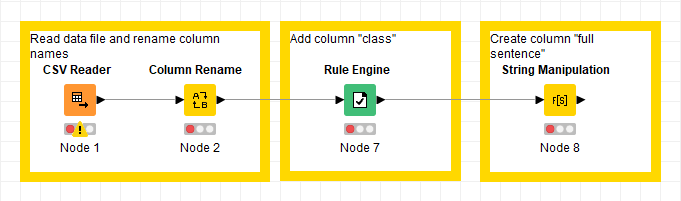
\includegraphics[scale=0.5]{images/workflow_ej1.png}
	\caption{Workflow del ejercicio 1}
	\label{fig:workflow_ej1}
\end{figure}

\section{Ejercicio 2}

Se va a proceder a analizar un conjunto de datos que describe el número de visitantes de un sitio web en los meses de junio/julio de 2010 (fichero \emph{website1.txt}).\\

Para calcular los parámetros de media, desviación típica, Kurtosis se ha utilizado el \emph{workflow} mostrado en la Figura \ref{fig:workflow_ej2}.\\
La \emph{Kurtosis} es una medida estadística que muestra la forma de una distribución de probabilidad. Una \emph{Kurtosis} grande implica una mayor concentración de valores de la variables o muy cerca de la media de la distribución (pico) o muy lejos de ella (colas de la distribución), al mismo tiempo que existe una menor frecuencia de valores intermedios.\\
Una \emph{Kurtosis} pequeña (como en este caso cuyo valor es 0.466) implica que los datos se establecen alrededor de la media, es decir, que el conjunto de datos no presenta \emph{datos atípicos}.\\

Para entrenar la red Bayesiana (Figura \ref{fig:workflow_ej2}) se deben preparar los datos. Para ello se debe crear una nueva columna \emph{isWeekend} para ilustrar si es fin de semana o no. Utilizando el nodo \emph{Rule engine} se utilizarán las siguientes reglas:

\begin{lstlisting}
$weekday$ MATCHES "Sat" => "Yes"
$weekday$ MATCHES "Sun" => "Yes"
TRUE => "No"
\end{lstlisting}

Se ha utilizado un nodo \emph{Column filter} para eliminar la columna \emph{weekday} ya que la red Bayesiana presenta un mejor rendimiento si conoce este valor ya que si se entrena con esta variable reconoce la regla de creación de la columna \emph{isWeekend}.\\
Para llegar a esta conclusión se han probado las distintas combinaciones de columnas utilizando el \emph{Column Filter}, eligiendo las columnas que se utilizarán para entrenar la red \emph{Bayesiana} y comparando con cual de ellas se obtiene un mejor rendimiento.\\

Para dibujar la curva \emph{ROC} se ha utilizado un nodo \emph{ROC Curve} a la salida del nodo \emph{Naive Bayes Predictor}. Se puede observar en la Figura \ref{fig:curvaROC_ej2} que la gráfica se encuentra mayoritariamente en la sección superior del triángulo. Esto indica que el modelo es capaz de identificar correctamente los verdaderos positivos. La curva \emph{ROC} se utiliza para estudiar la sensibilidad y la especialidad de un test diagnóstico.\\


\begin{figure}[h!]
	\centering
	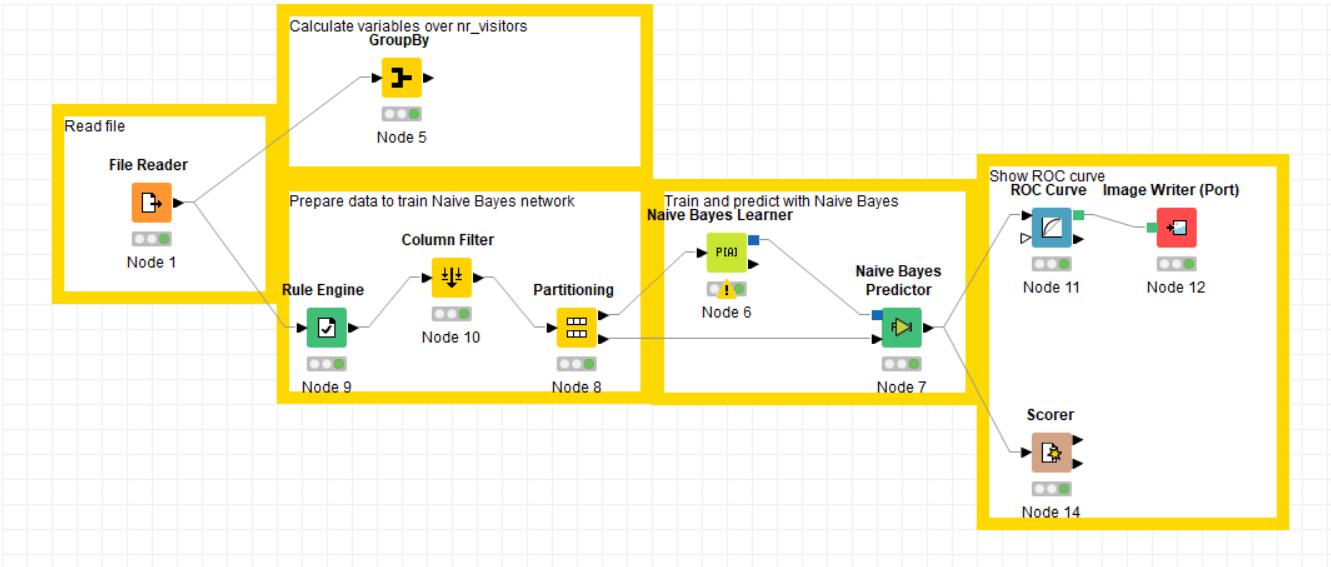
\includegraphics[scale=0.5]{images/workflow_ej2.png}
	\caption{Workflow de ejercicio 2}
	\label{fig:workflow_ej2}
\end{figure}

\begin{figure}[h!]
	\centering
	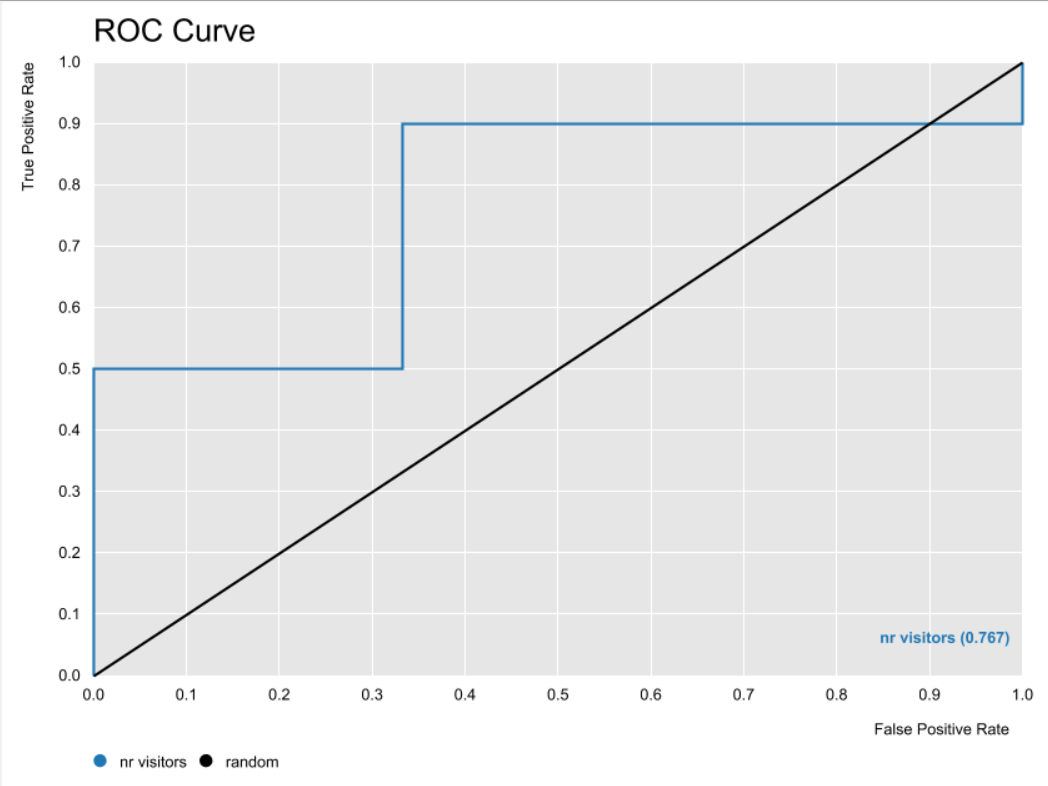
\includegraphics[scale=0.5]{images/curva_ROC.png}
	\caption{Curva ROC del ejercicio 2}
	\label{fig:curvaROC_ej2}
\end{figure}


\section{Ejercicio 3}

Para la evaluación de los distintos conjuntos de datos se han creado 2 \emph{workflows}. Uno de ellos (Figura \ref{fig:workflow_knime}) utiliza las herramientas de \emph{KNIME} para evaluar los datos. El otro (Figura \ref{fig:workflow_weka}) utiliza las herramientas de \emph{WEKA} para evaluar los datos.\\
En el anexo se pueden observar las tablas comparativas de las distintas ejecuciones de los \emph{workflows} tanto con \emph{KNIME} (K) como con \emph{WEKA} (W).\\
Para el conjunto de datos \emph{wine} se han entrenado las distintas herramientas con el 80\%, 50\% y 30\%.\\
Para el conjunto de datos \emph{wine} se han entrenado las distintas herramientas con el 80\%, 50\% y 30\%.
Se puede apreciar que conforme se reduce el número de datos de entrenamiento se pierde precisión, aunque de de una manera muy ligera ya que no es un conjunto grande de datos ni se ha ejecutado una cantidad grande de veces para que se estabilicen los resultados. El método que mejor ha funcionado identificando de las clases ha sido el perceptrón multicapa, ya que se ha utilizado la configuración del perceptrón que mejor funcionaba en la anterior práctica.\\
Cabe destacar que tanto el perceptrón multicapa como Naive Bayes realizan una clasificación del tipo 3 muy correcta, pero J48 erra bastante con respecto a los dos anteriores, prácticamente siempre por debajo del 0.9 de TP.\\

Para el conjunto de datos \emph{iris} se han entrenado las distintas herramientas con el 80\%, 50\% y 30\% de los datos.\\ Se puede observar que en todos los modelos se obtienen los resultados más precisos cuando se usa un mayor número de datos de entrenamiento (80\%), llegando en algunos casos a clasificar correctamente el 100\% de los elementos pertenecientes a la clase \textit{Iris-Setosa}, ya que la tasa de \textit{True Positives} es 1.\par
Los peores resultados se han obtenido con el modelo de \textit{perteptrón multicapa}, sobre todo con los nodos de \textit{Knime}, ya que la media de \textit{True Positives} ronda el 80\% para cada una de las clases.
La mayor tasa de \textit{True Positives} se ha obtenido con el modelo \textit{J48}, sobre todo con los nodos de \textit{Knime}, ya que se obtiene una media de \textit{True Positives} superior al 90\% para cada una de las clases, llegando incluso al 100\% para la clase \textit{Iris-Setosa}. El modelo \textit{Naive Bayes} consigue unos resultados muy parecidos al de \textit{J48}, sobre todo con los nodos de \textit{Weka}.\\

Para el conjunto de datos \emph{adult} se han entrenado las distintas herramientas con el 80\%, 50\% y 30\%.
Se puede apreciar que conforme se reduce el número de datos de entrenamiento se pierde precisión, identificando datos pertenecientes a la otra clase de datos ($>$50K) como datos de clase $<=$50K. El método que más ha errado en la identificación de las clases ha sido el perceptrón multicapa.\\
El método que menos ha variado la precisión conforme se entrenaba con menos datos ha sido el \emph{J48} y en especial utilizando los nodos de \emph{WEKA} siempre ha mantenido el porcentaje de \emph{True Positives} por encima del 93\% en la clase $<=$50K y del 60\% en la clase $>$50K.\\

Se ha planteado una gráfica (Figura \ref{fig:graficaComparativa}) para el conjunto de datos \emph{Iris} en la cual se compara la precisión de los distintos métodos conforme se van reduciendo los datos de entrenamiento. Se puede observar un descenso de la precisión en las clases \emph{Iris-Versicolor} e \emph{Iris-Virgínica} conforme se reducen los datos. Se puede observar como el perceptrón no varía especialmente conforme se reducen los datos de entrenamiento. Este fenómeno puede ocurrir debido a que el particionado de los datos se ha realizado de forma aleatoria con el nodo \emph{partitioning} y se han realizado 5 ejecuciones para hallar una media en la precisión de la identificación de las clases.\\

\begin{figure}[h!]
	\centering
	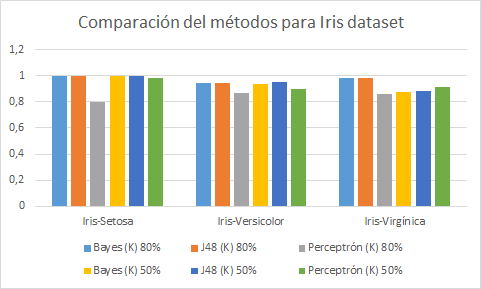
\includegraphics[scale=0.9]{images/comparacionMetodos.png}
	\caption{Gráfica comparativa de los métodos para el dataset \emph{Iris}}
	\label{fig:graficaComparativa}
\end{figure}


En cuanto a los problemas que han surgido, con el \emph{dataset} \emph{adult} se necesitaba una columna \emph{Class} y por lo tanto, se ha renombrado la última columna a \emph{``Class''}. Para ello se ha utilizado un nodo \emph{Column Filter} para eliminar todas las variables no numéricas (a excepción de la columna \emph{``Class''}).\\

Para simplificar y agilizar el entrenamiento y ejecución de cada uno de los clasificadores, se han creado dos \textit{workflows}, uno que agrupa todos los clasificadores que provee la propia herramienta \textit{Knime} (Figura \ref{fig:workflow_knime}) y otro que agrupa los nodos que proporciona el \textit{plugin} de \textit{Weka} (Figura \ref{fig:workflow_weka}).\\


\begin{figure}[h!]
	\centering
	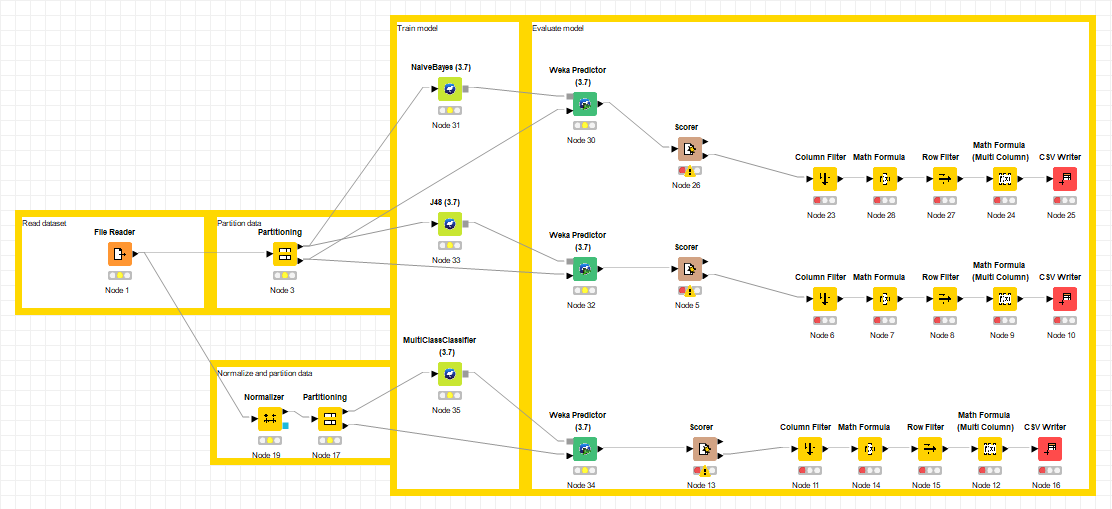
\includegraphics[scale=0.5]{images/workflow_ej3_weka.png}
	\caption{Workflow con modelos de entrenamiento de \textit{Weka}}
	\label{fig:workflow_weka}
\end{figure}


\begin{figure}[h!]
	\centering
	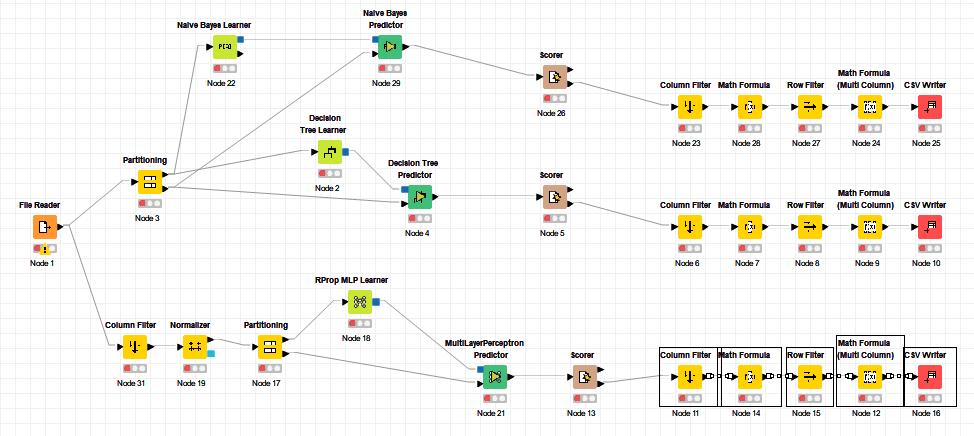
\includegraphics[scale=0.5]{images/workflow_ej3_knime.png}
	\caption{Workflow con modelos de entrenamiento de \textit{Knime}}
	\label{fig:workflow_knime}
\end{figure}

De esta manera en cada \textit{Workflow} se indica el \textit{dataset} deseado con el nodo \textit{File Reader} y se selecciona el porcentaje de datos a entrenar con el nodo \textit{partitioning}. Los resultados se escriben en archivos \textit{csv} distintos, indicados con los nodos \textit{CSV Writer}. Así se centralizan los diferentes modelos de entrenamiento con una sola ejecución.\\

\newpage
\section{Anexo 1: Cuadros de datos ejercicio 3}

\subsection{Dataset Adult}

\subsubsection{Naive Bayes}
\begin{table}[h]
\begin{tabular}{lllll}
\hline
\multicolumn{1}{|c|}{\textbf{Clase}} & \multicolumn{1}{c|}{\textbf{True Positives (K)}} & \multicolumn{1}{c|}{\textbf{False Positives (K)}} & \multicolumn{1}{c|}{\textbf{True Positives (W)}} & \multicolumn{1}{l|}{\textbf{False Positives (W)}} \\ \hline
\multicolumn{1}{|l|}{\textbf{$<=$50K}} & \multicolumn{1}{l|}{0.942}          & \multicolumn{1}{l|}{0.058}          & \multicolumn{1}{l|}{0.936}          & \multicolumn{1}{l|}{0.064} \\ \hline
\multicolumn{1}{|l|}{\textbf{$>$50K}} & \multicolumn{1}{l|}{0.511}          & \multicolumn{1}{l|}{0.489}          & \multicolumn{1}{l|}{0.515}          & \multicolumn{1}{l|}{0.485} \\ \hline
\textbf{}                       &                                &                                &                                &                      
\end{tabular}
\caption{Datos de entrenamiento del dataset \emph{Adult} con el 80\% usando \emph{Naive Bayes}}
\label{tab:adult_bayes_80}
\end{table}

\begin{table}[h]
\begin{tabular}{lllll}
\hline
\multicolumn{1}{|c|}{\textbf{Clase}} & \multicolumn{1}{c|}{\textbf{True Positives (K)}} & \multicolumn{1}{c|}{\textbf{False Positives (K)}} & \multicolumn{1}{c|}{\textbf{True Positives (W)}} & \multicolumn{1}{l|}{\textbf{False Positives (W)}} \\ \hline
\multicolumn{1}{|l|}{\textbf{$<=$50K}} & \multicolumn{1}{l|}{0.941}          & \multicolumn{1}{l|}{0.059}          & \multicolumn{1}{l|}{0.933}          & \multicolumn{1}{l|}{0.067} \\ \hline
\multicolumn{1}{|l|}{\textbf{$>$50K}} & \multicolumn{1}{l|}{0.513}          & \multicolumn{1}{l|}{0.487}          & \multicolumn{1}{l|}{0.513}          & \multicolumn{1}{l|}{0.487} \\ \hline
\textbf{}                       &                                &                                &                                &                      
\end{tabular}
\caption{Datos de entrenamiento del dataset \emph{Adult} con el 50\% usando \emph{Naive Bayes}}
\label{tab:adult_bayes_50}
\end{table}

\begin{table}[h!]
\begin{tabular}{lllll}
\hline
\multicolumn{1}{|c|}{\textbf{Clase}} & \multicolumn{1}{c|}{\textbf{True Positives (K)}} & \multicolumn{1}{c|}{\textbf{False Positives (K)}} & \multicolumn{1}{c|}{\textbf{True Positives (W)}} & \multicolumn{1}{l|}{\textbf{False Positives (W)}} \\ \hline
\multicolumn{1}{|l|}{\textbf{$<=$50K}} & \multicolumn{1}{l|}{0.939}          & \multicolumn{1}{l|}{0.061}          & \multicolumn{1}{l|}{0.934}          & \multicolumn{1}{l|}{0.066} \\ \hline
\multicolumn{1}{|l|}{\textbf{$>$50K}} & \multicolumn{1}{l|}{0.508}          & \multicolumn{1}{l|}{0.492}          & \multicolumn{1}{l|}{0.522}          & \multicolumn{1}{l|}{0.478} \\ \hline
\textbf{}                       &                                &                                &                                &                      
\end{tabular}
\caption{Datos de entrenamiento del dataset \emph{Adult} con el 30\% usando \emph{Naive Bayes}}
\label{tab:adult_bayes_30}
\end{table}

\newpage
\subsubsection{J48}

\begin{table}[h]
\begin{tabular}{lllll}
\hline
\multicolumn{1}{|c|}{\textbf{Clase}} & \multicolumn{1}{c|}{\textbf{True Positives (K)}} & \multicolumn{1}{c|}{\textbf{False Positives (K)}} & \multicolumn{1}{c|}{\textbf{True Positives (W)}} & \multicolumn{1}{l|}{\textbf{False Positives (W)}} \\ \hline
\multicolumn{1}{|l|}{\textbf{$<=$50K}} & \multicolumn{1}{l|}{0.900}          & \multicolumn{1}{l|}{0.100}          & \multicolumn{1}{l|}{0.936}          & \multicolumn{1}{l|}{0.064} \\ \hline
\multicolumn{1}{|l|}{\textbf{$>$50K}} & \multicolumn{1}{l|}{0.603}          & \multicolumn{1}{l|}{0.397}          & \multicolumn{1}{l|}{0.621}          & \multicolumn{1}{l|}{0.379} \\ \hline
\textbf{}                       &                                &                                &                                &                      
\end{tabular}
\caption{Datos de entrenamiento del dataset \emph{Adult} con el 80\% usando \emph{J48}}
\label{tab:adult_j48_80}
\end{table}

\begin{table}[h]
\begin{tabular}{lllll}
\hline
\multicolumn{1}{|c|}{\textbf{Clase}} & \multicolumn{1}{c|}{\textbf{True Positives (K)}} & \multicolumn{1}{c|}{\textbf{False Positives (K)}} & \multicolumn{1}{c|}{\textbf{True Positives (W)}} & \multicolumn{1}{l|}{\textbf{False Positives (W)}} \\ \hline
\multicolumn{1}{|l|}{\textbf{$<=$50K}} & \multicolumn{1}{l|}{0.897}          & \multicolumn{1}{l|}{0.103}          & \multicolumn{1}{l|}{0.937}          & \multicolumn{1}{l|}{0.063} \\ \hline
\multicolumn{1}{|l|}{\textbf{$>$50K}} & \multicolumn{1}{l|}{0.598}          & \multicolumn{1}{l|}{0.402}          & \multicolumn{1}{l|}{0.607}          & \multicolumn{1}{l|}{0.392} \\ \hline
\textbf{}                       &                                &                                &                                &                      
\end{tabular}
\caption{Datos de entrenamiento del dataset \emph{Adult} con el 50\% usando \emph{J48}}
\label{tab:adult_j48_50}
\end{table}

\begin{table}[h]
\begin{tabular}{lllll}
\hline
\multicolumn{1}{|c|}{\textbf{Clase}} & \multicolumn{1}{c|}{\textbf{True Positives (K)}} & \multicolumn{1}{c|}{\textbf{False Positives (K)}} & \multicolumn{1}{c|}{\textbf{True Positives (W)}} & \multicolumn{1}{l|}{\textbf{False Positives (W)}} \\ \hline
\multicolumn{1}{|l|}{\textbf{$<=$50K}} & \multicolumn{1}{l|}{0.890}          & \multicolumn{1}{l|}{0.110}          & \multicolumn{1}{l|}{0.933}          & \multicolumn{1}{l|}{0.067} \\ \hline
\multicolumn{1}{|l|}{\textbf{$>$50K}} & \multicolumn{1}{l|}{0.599}          & \multicolumn{1}{l|}{0.401}          & \multicolumn{1}{l|}{0.600}          & \multicolumn{1}{l|}{0.400} \\ \hline
\textbf{}                       &                                &                                &                                &                      
\end{tabular}
\caption{Datos de entrenamiento del dataset \emph{Adult} con el 30\% usando \emph{J48}}
\label{tab:adult_j48_30}
\end{table}

\newpage
\subsubsection{Perceptrón multicapa}
\begin{table}[h]
\begin{tabular}{lllll}
\hline
\multicolumn{1}{|c|}{\textbf{Clase}} & \multicolumn{1}{c|}{\textbf{True Positives (K)}} & \multicolumn{1}{c|}{\textbf{False Positives (K)}} & \multicolumn{1}{c|}{\textbf{True Positives (W)}} & \multicolumn{1}{l|}{\textbf{False Positives (W)}} \\ \hline
\multicolumn{1}{|l|}{\textbf{$<=$50K}} & \multicolumn{1}{l|}{0.901}          & \multicolumn{1}{l|}{0.099}          & \multicolumn{1}{l|}{0.927}          & \multicolumn{1}{l|}{0.073} \\ \hline
\multicolumn{1}{|l|}{\textbf{$>$50K}} & \multicolumn{1}{l|}{0.377}          & \multicolumn{1}{l|}{0.623}          & \multicolumn{1}{l|}{0.602}          & \multicolumn{1}{l|}{0.398} \\ \hline
\textbf{}                       &                                &                                &                                &                      
\end{tabular}
\caption{Datos de entrenamiento del dataset \emph{Adult} con el 80\% usando \emph{Perceptrón multicapa}}
\label{tab:adult_perceptron_80}
\end{table}

\begin{table}[h!]
\begin{tabular}{lllll}
\hline
\multicolumn{1}{|c|}{\textbf{Clase}} & \multicolumn{1}{c|}{\textbf{True Positives (K)}} & \multicolumn{1}{c|}{\textbf{False Positives (K)}} & \multicolumn{1}{c|}{\textbf{True Positives (W)}} & \multicolumn{1}{l|}{\textbf{False Positives (W)}} \\ \hline
\multicolumn{1}{|l|}{\textbf{$<=$50K}} & \multicolumn{1}{l|}{1.000}          & \multicolumn{1}{l|}{0.000}          & \multicolumn{1}{l|}{0.930}          & \multicolumn{1}{l|}{0.070} \\ \hline
\multicolumn{1}{|l|}{\textbf{$>$50K}} & \multicolumn{1}{l|}{0.000}          & \multicolumn{1}{l|}{1.000}          & \multicolumn{1}{l|}{0.605}          & \multicolumn{1}{l|}{0.395} \\ \hline
\textbf{}                       &                                &                                &                                &                      
\end{tabular}
\caption{Datos de entrenamiento del dataset \emph{Adult} con el 50\% usando \emph{Perceptrón multicapa}}
\label{tab:adult_perceptron_50}
\end{table}

\begin{table}[h!]
\begin{tabular}{lllll}
\hline
\multicolumn{1}{|c|}{\textbf{Clase}} & \multicolumn{1}{c|}{\textbf{True Positives (K)}} & \multicolumn{1}{c|}{\textbf{False Positives (K)}} & \multicolumn{1}{c|}{\textbf{True Positives (W)}} & \multicolumn{1}{l|}{\textbf{False Positives (W)}} \\ \hline
\multicolumn{1}{|l|}{\textbf{$<=$50K}} & \multicolumn{1}{l|}{0.890}          & \multicolumn{1}{l|}{0.110}          & \multicolumn{1}{l|}{0.932}          & \multicolumn{1}{l|}{0.068} \\ \hline
\multicolumn{1}{|l|}{\textbf{$>$50K}} & \multicolumn{1}{l|}{0.389}          & \multicolumn{1}{l|}{0.611}          & \multicolumn{1}{l|}{0.587}          & \multicolumn{1}{l|}{0.413} \\ \hline
\textbf{}                       &                                &                                &                                &                      
\end{tabular}
\caption{Datos de entrenamiento del dataset \emph{Adult} con el 30\% usando \emph{Perceptrón multicapa}}
\label{tab:adult_perceptron_30}
\end{table}

\newpage
\subsection{Dataset Iris}
\subsubsection{Naive Bayes}
\begin{table}[h!]
	\begin{tabular}{lllll}
		\hline
		\multicolumn{1}{|c|}{\textbf{Clase}} & \multicolumn{1}{c|}{\textbf{True Positives (K)}} & \multicolumn{1}{c|}{\textbf{False Positives (K)}} & \multicolumn{1}{c|}{\textbf{True Positives (W)}} & \multicolumn{1}{l|}{\textbf{False Positives (W)}} \\ \hline
		\multicolumn{1}{|l|}{\textbf{Iris-Setosa}} & \multicolumn{1}{l|}{1}          & \multicolumn{1}{l|}{0}          & \multicolumn{1}{l|}{1}          & \multicolumn{1}{l|}{0} \\ \hline
		\multicolumn{1}{|l|}{\textbf{Iris-versicolor}} & \multicolumn{1}{l|}{0,947}          & \multicolumn{1}{l|}{0,053}          & \multicolumn{1}{l|}{0,928}          & \multicolumn{1}{l|}{0,072} \\ \hline
		\multicolumn{1}{|l|}{\textbf{Iris-virginica}} & \multicolumn{1}{l|}{0,983}          & \multicolumn{1}{l|}{0,017}          & \multicolumn{1}{l|}{0,913}          & \multicolumn{1}{l|}{0,087}\\ \hline
		\textbf{}                       &                                &                                &                                &                      
 
	\end{tabular}
	\caption{Datos de entrenamiento del dataset \emph{Iris} con el 80\% usando \emph{Naive Bayes}}
	\label{tab:iris_bayes_80}
\end{table}

\begin{table}[h!]
	\begin{tabular}{lllll}
		\hline
		\multicolumn{1}{|c|}{\textbf{Clase}} & \multicolumn{1}{c|}{\textbf{True Positives (K)}} & \multicolumn{1}{c|}{\textbf{False Positives (K)}} & \multicolumn{1}{c|}{\textbf{True Positives (W)}} & \multicolumn{1}{l|}{\textbf{False Positives (W)}} \\ \hline
		\multicolumn{1}{|l|}{\textbf{Iris-Setosa}} & \multicolumn{1}{l|}{1}          & \multicolumn{1}{l|}{0}          & \multicolumn{1}{l|}{1}          & \multicolumn{1}{l|}{0} \\ \hline
		\multicolumn{1}{|l|}{\textbf{Iris-versicolor}} & \multicolumn{1}{l|}{0,938}          & \multicolumn{1}{l|}{0,062}          & \multicolumn{1}{l|}{0,895}          & \multicolumn{1}{l|}{0,105} \\ \hline
		\multicolumn{1}{|l|}{\textbf{Iris-virginica}} & \multicolumn{1}{l|}{0,874}          & \multicolumn{1}{l|}{0,126}          & \multicolumn{1}{l|}{0,912}          & \multicolumn{1}{l|}{0,088}\\ \hline
		\textbf{}                       &                                &                                &                                &                      
		
	\end{tabular}
	\caption{Datos de entrenamiento del dataset \emph{Iris} con el 50\% usando \emph{Naive Bayes}}
	\label{tab:iris_bayes_50}
\end{table}


\begin{table}[h!]
	\begin{tabular}{lllll}
		\hline
		\multicolumn{1}{|c|}{\textbf{Clase}} & \multicolumn{1}{c|}{\textbf{True Positives (K)}} & \multicolumn{1}{c|}{\textbf{False Positives (K)}} & \multicolumn{1}{c|}{\textbf{True Positives (W)}} & \multicolumn{1}{l|}{\textbf{False Positives (W)}} \\ \hline
		\multicolumn{1}{|l|}{\textbf{Iris-Setosa}} & \multicolumn{1}{l|}{1}          & \multicolumn{1}{l|}{0}          & \multicolumn{1}{l|}{1}          & \multicolumn{1}{l|}{0} \\ \hline
		\multicolumn{1}{|l|}{\textbf{Iris-versicolor}} & \multicolumn{1}{l|}{0,904}          & \multicolumn{1}{l|}{0,096}          & \multicolumn{1}{l|}{0,814}          & \multicolumn{1}{l|}{0,186} \\ \hline
		\multicolumn{1}{|l|}{\textbf{Iris-virginica}} & \multicolumn{1}{l|}{0,883}          & \multicolumn{1}{l|}{0,117}          & \multicolumn{1}{l|}{0,932}          & \multicolumn{1}{l|}{0,068}\\ \hline
		\textbf{}                       &                                &                                &                                &                      
		
	\end{tabular}
	\caption{Datos de entrenamiento del dataset \emph{Iris} con el 30\% usando \emph{Naive Bayes}}
	\label{tab:iris_bayes_30}
\end{table}
\newpage
\subsubsection{J48}
\begin{table}[h!]
	\begin{tabular}{lllll}
		\hline
		\multicolumn{1}{|c|}{\textbf{Clase}} & \multicolumn{1}{c|}{\textbf{True Positives (K)}} & \multicolumn{1}{c|}{\textbf{False Positives (K)}} & \multicolumn{1}{c|}{\textbf{True Positives (W)}} & \multicolumn{1}{l|}{\textbf{False Positives (W)}} \\ \hline
		\multicolumn{1}{|l|}{\textbf{Iris-Setosa}} & \multicolumn{1}{l|}{1}          & \multicolumn{1}{l|}{0}          & \multicolumn{1}{l|}{1}          & \multicolumn{1}{l|}{0} \\ \hline
		\multicolumn{1}{|l|}{\textbf{Iris-versicolor}} & \multicolumn{1}{l|}{0,947}          & \multicolumn{1}{l|}{0,053}          & \multicolumn{1}{l|}{0,903}          & \multicolumn{1}{l|}{0,097} \\ \hline
		\multicolumn{1}{|l|}{\textbf{Iris-virginica}} & \multicolumn{1}{l|}{0,983}          & \multicolumn{1}{l|}{0,017}          & \multicolumn{1}{l|}{0,910}          & \multicolumn{1}{l|}{0,090}\\ \hline
		\textbf{}                       &                                &                                &                                &                      
		
	\end{tabular}
	\caption{Datos de entrenamiento del dataset \emph{Iris} con el 80\% usando \emph{J48}}
	\label{tab:iris_j48_80}
\end{table}

\begin{table}[h!]
	\begin{tabular}{lllll}
		\hline
		\multicolumn{1}{|c|}{\textbf{Clase}} & \multicolumn{1}{c|}{\textbf{True Positives (K)}} & \multicolumn{1}{c|}{\textbf{False Positives (K)}} & \multicolumn{1}{c|}{\textbf{True Positives (W)}} & \multicolumn{1}{l|}{\textbf{False Positives (W)}} \\ \hline
		\multicolumn{1}{|l|}{\textbf{Iris-Setosa}} & \multicolumn{1}{l|}{1}          & \multicolumn{1}{l|}{0}          & \multicolumn{1}{l|}{0,968}          & \multicolumn{1}{l|}{0,032} \\ \hline
		\multicolumn{1}{|l|}{\textbf{Iris-versicolor}} & \multicolumn{1}{l|}{0,952}          & \multicolumn{1}{l|}{0,048}          & \multicolumn{1}{l|}{0,909}          & \multicolumn{1}{l|}{0,091} \\ \hline
		\multicolumn{1}{|l|}{\textbf{Iris-virginica}} & \multicolumn{1}{l|}{0,886}          & \multicolumn{1}{l|}{0,114}          & \multicolumn{1}{l|}{0,885}          & \multicolumn{1}{l|}{0,115}\\ \hline
		\textbf{}                       &                                &                                &                                &                      
		
	\end{tabular}
	\caption{Datos de entrenamiento del dataset \emph{Iris} con el 50\% usando \emph{J48}}
	\label{tab:iris_j48_50}
\end{table}

\begin{table}[h!]
	\begin{tabular}{lllll}
		\hline
		\multicolumn{1}{|c|}{\textbf{Clase}} & \multicolumn{1}{c|}{\textbf{True Positives (K)}} & \multicolumn{1}{c|}{\textbf{False Positives (K)}} & \multicolumn{1}{c|}{\textbf{True Positives (W)}} & \multicolumn{1}{l|}{\textbf{False Positives (W)}} \\ \hline
		\multicolumn{1}{|l|}{\textbf{Iris-Setosa}} & \multicolumn{1}{l|}{1}          & \multicolumn{1}{l|}{0}          & \multicolumn{1}{l|}{0,922}          & \multicolumn{1}{l|}{0,078} \\ \hline
		\multicolumn{1}{|l|}{\textbf{Iris-versicolor}} & \multicolumn{1}{l|}{0,935}          & \multicolumn{1}{l|}{0,065}          & \multicolumn{1}{l|}{0,910}          & \multicolumn{1}{l|}{0,090} \\ \hline
		\multicolumn{1}{|l|}{\textbf{Iris-virginica}} & \multicolumn{1}{l|}{0,907}          & \multicolumn{1}{l|}{0,093}          & \multicolumn{1}{l|}{0,942}          & \multicolumn{1}{l|}{0,058}\\ \hline
		\textbf{}                       &                                &                                &                                &                      
		
	\end{tabular}
	\caption{Datos de entrenamiento del dataset \emph{Iris} con el 30\% usando \emph{J48}}
	\label{tab:iris_j48_30}
\end{table}
\subsubsection{Perceptrón multicapa}
\begin{table}[h!]
	\begin{tabular}{lllll}
		\hline
		\multicolumn{1}{|c|}{\textbf{Clase}} & \multicolumn{1}{c|}{\textbf{True Positives (K)}} & \multicolumn{1}{c|}{\textbf{False Positives (K)}} & \multicolumn{1}{c|}{\textbf{True Positives (W)}} & \multicolumn{1}{l|}{\textbf{False Positives (W)}} \\ \hline
		\multicolumn{1}{|l|}{\textbf{Iris-Setosa}} & \multicolumn{1}{l|}{0,8}          & \multicolumn{1}{l|}{0,2}          & \multicolumn{1}{l|}{1}          & \multicolumn{1}{l|}{0} \\ \hline
		\multicolumn{1}{|l|}{\textbf{Iris-versicolor}} & \multicolumn{1}{l|}{0,865}          & \multicolumn{1}{l|}{0,135}          & \multicolumn{1}{l|}{0,883}          & \multicolumn{1}{l|}{0,117} \\ \hline
		\multicolumn{1}{|l|}{\textbf{Iris-virginica}} & \multicolumn{1}{l|}{0,860}          & \multicolumn{1}{l|}{0,140}          & \multicolumn{1}{l|}{0,822}          & \multicolumn{1}{l|}{0,178}\\ \hline
		\textbf{}                       &                                &                                &                                &                      
		
	\end{tabular}
	\caption{Datos de entrenamiento del dataset \emph{Iris} con el 80\% usando \emph{Perceptrón multicapa}}
	\label{tab:iris_percep_80}
\end{table}

\begin{table}[h!]
	\begin{tabular}{lllll}
		\hline
		\multicolumn{1}{|c|}{\textbf{Clase}} & \multicolumn{1}{c|}{\textbf{True Positives (K)}} & \multicolumn{1}{c|}{\textbf{False Positives (K)}} & \multicolumn{1}{c|}{\textbf{True Positives (W)}} & \multicolumn{1}{l|}{\textbf{False Positives (W)}} \\ \hline
		\multicolumn{1}{|l|}{\textbf{Iris-Setosa}} & \multicolumn{1}{l|}{0,984}          & \multicolumn{1}{l|}{0,016}          & \multicolumn{1}{l|}{1}          & \multicolumn{1}{l|}{0} \\ \hline
		\multicolumn{1}{|l|}{\textbf{Iris-versicolor}} & \multicolumn{1}{l|}{0,898}          & \multicolumn{1}{l|}{0,102}          & \multicolumn{1}{l|}{0,933}          & \multicolumn{1}{l|}{0,066} \\ \hline
		\multicolumn{1}{|l|}{\textbf{Iris-virginica}} & \multicolumn{1}{l|}{0,915}          & \multicolumn{1}{l|}{0,085}          & \multicolumn{1}{l|}{0,947}          & \multicolumn{1}{l|}{0,053}\\ \hline
		\textbf{}                       &                                &                                &                                &                      
		
	\end{tabular}
	\caption{Datos de entrenamiento del dataset \emph{Iris} con el 50\% usando \emph{Perceptrón multicapa}}
	\label{tab:iris_percep_50}
\end{table}

\begin{table}[h!]
	\begin{tabular}{lllll}
		\hline
		\multicolumn{1}{|c|}{\textbf{Clase}} & \multicolumn{1}{c|}{\textbf{True Positives (K)}} & \multicolumn{1}{c|}{\textbf{False Positives (K)}} & \multicolumn{1}{c|}{\textbf{True Positives (W)}} & \multicolumn{1}{l|}{\textbf{False Positives (W)}} \\ \hline
		\multicolumn{1}{|l|}{\textbf{Iris-Setosa}} & \multicolumn{1}{l|}{0,995}          & \multicolumn{1}{l|}{0,005}          & \multicolumn{1}{l|}{0,995}          & \multicolumn{1}{l|}{0,005} \\ \hline
		\multicolumn{1}{|l|}{\textbf{Iris-versicolor}} & \multicolumn{1}{l|}{0,797}          & \multicolumn{1}{l|}{0,203}          & \multicolumn{1}{l|}{0,885}          & \multicolumn{1}{l|}{0,115} \\ \hline
		\multicolumn{1}{|l|}{\textbf{Iris-virginica}} & \multicolumn{1}{l|}{0,853}          & \multicolumn{1}{l|}{0,147}          & \multicolumn{1}{l|}{0,832}          & \multicolumn{1}{l|}{0,168}\\ \hline
		\textbf{}                       &                                &                                &                                &                      
		
	\end{tabular}
	\caption{Datos de entrenamiento del dataset \emph{Iris} con el 30\% usando \emph{Perceptrón multicapa}}
	\label{tab:iris_percep_30}
\end{table}

\newpage
\subsection{Dataset Wine}

\subsubsection{Naive Bayes}
\begin{table}[h!]
	\begin{tabular}{lllll}
		\hline
		\multicolumn{1}{|c|}{\textbf{Clase}} & \multicolumn{1}{c|}{\textbf{True Positives (K)}} & \multicolumn{1}{c|}{\textbf{False Positives (K)}} & \multicolumn{1}{c|}{\textbf{True Positives (W)}} & \multicolumn{1}{l|}{\textbf{False Positives (W)}} \\ \hline
		\multicolumn{1}{|l|}{\textbf{1}} & \multicolumn{1}{l|}{0,968}          & \multicolumn{1}{l|}{0,031}          & \multicolumn{1}{l|}{0,966}          & \multicolumn{1}{l|}{0,033} \\ \hline
		\multicolumn{1}{|l|}{\textbf{2}} & \multicolumn{1}{l|}{0,959}          & \multicolumn{1}{l|}{0,040}          & \multicolumn{1}{l|}{0,939}          & \multicolumn{1}{l|}{0,060} \\ \hline
		\multicolumn{1}{|l|}{\textbf{3}} & \multicolumn{1}{l|}{0,984}          & \multicolumn{1}{l|}{0,015}          & \multicolumn{1}{l|}{1}          & \multicolumn{1}{l|}{0}\\ \hline
		\textbf{}                       &                                &                                &                                &                      
 
	\end{tabular}
	\caption{Datos de entrenamiento del dataset \emph{Wine} con el 80\% usando \emph{Naive Bayes}}
	\label{tab:wine_bayes_80}
\end{table}

\begin{table}[h!]
	\begin{tabular}{lllll}
		\hline
		\multicolumn{1}{|c|}{\textbf{Clase}} & \multicolumn{1}{c|}{\textbf{True Positives (K)}} & \multicolumn{1}{c|}{\textbf{False Positives (K)}} & \multicolumn{1}{c|}{\textbf{True Positives (W)}} & \multicolumn{1}{l|}{\textbf{False Positives (W)}} \\ \hline
		\multicolumn{1}{|l|}{\textbf{1}} & \multicolumn{1}{l|}{0,961}          & \multicolumn{1}{l|}{0,038}          & \multicolumn{1}{l|}{0,956}          & \multicolumn{1}{l|}{0,043} \\ \hline
		\multicolumn{1}{|l|}{\textbf{2}} & \multicolumn{1}{l|}{0,953}          & \multicolumn{1}{l|}{0,056}          & \multicolumn{1}{l|}{0,943}          & \multicolumn{1}{l|}{0,105} \\ \hline
		\multicolumn{1}{|l|}{\textbf{3}} & \multicolumn{1}{l|}{1}          & \multicolumn{1}{l|}{0}          & \multicolumn{1}{l|}{1}          & \multicolumn{1}{l|}{1}\\ \hline
		\textbf{}                       &                                &                                &                                &                      
		
	\end{tabular}
	\caption{Datos de entrenamiento del dataset \emph{Wine} con el 50\% usando \emph{Naive Bayes}}
	\label{tab:wine_bayes_50}
\end{table}


\begin{table}[h!]
	\begin{tabular}{lllll}
		\hline
		\multicolumn{1}{|c|}{\textbf{Clase}} & \multicolumn{1}{c|}{\textbf{True Positives (K)}} & \multicolumn{1}{c|}{\textbf{False Positives (K)}} & \multicolumn{1}{c|}{\textbf{True Positives (W)}} & \multicolumn{1}{l|}{\textbf{False Positives (W)}} \\ \hline
		\multicolumn{1}{|l|}{\textbf{1}} & \multicolumn{1}{l|}{0,955}          & \multicolumn{1}{l|}{0,044}          & \multicolumn{1}{l|}{0,978}          & \multicolumn{1}{l|}{0,021} \\ \hline
		\multicolumn{1}{|l|}{\textbf{2}} & \multicolumn{1}{l|}{0,946}          & \multicolumn{1}{l|}{0,053}          & \multicolumn{1}{l|}{0,944}          & \multicolumn{1}{l|}{0,055} \\ \hline
		\multicolumn{1}{|l|}{\textbf{3}} & \multicolumn{1}{l|}{0,994}          & \multicolumn{1}{l|}{0,005}          & \multicolumn{1}{l|}{0,983}          & \multicolumn{1}{l|}{0,016}\\ \hline
		\textbf{}                       &                                &                                &                                &                      
		
	\end{tabular}
	\caption{Datos de entrenamiento del dataset \emph{Wine} con el 30\% usando \emph{Naive Bayes}}
	\label{tab:wine_bayes_30}
\end{table}
\newpage
\subsubsection{J48}
\begin{table}[h!]
	\begin{tabular}{lllll}
		\hline
		\multicolumn{1}{|c|}{\textbf{Clase}} & \multicolumn{1}{c|}{\textbf{True Positives (K)}} & \multicolumn{1}{c|}{\textbf{False Positives (K)}} & \multicolumn{1}{c|}{\textbf{True Positives (W)}} & \multicolumn{1}{l|}{\textbf{False Positives (W)}} \\ \hline
		\multicolumn{1}{|l|}{\textbf{1}} & \multicolumn{1}{l|}{0,941}          & \multicolumn{1}{l|}{0,058}          & \multicolumn{1}{l|}{0,984}          & \multicolumn{1}{l|}{0,015} \\ \hline
		\multicolumn{1}{|l|}{\textbf{2}} & \multicolumn{1}{l|}{0,887}          & \multicolumn{1}{l|}{0,112}          & \multicolumn{1}{l|}{0,923}          & \multicolumn{1}{l|}{0,076} \\ \hline
		\multicolumn{1}{|l|}{\textbf{3}} & \multicolumn{1}{l|}{0,860}          & \multicolumn{1}{l|}{0,139}          & \multicolumn{1}{l|}{0,969}          & \multicolumn{1}{l|}{0,030}\\ \hline
		\textbf{}                       &                                &                                &                                &                      
		
	\end{tabular}
	\caption{Datos de entrenamiento del dataset \emph{Wine} con el 80\% usando \emph{J48}}
	\label{tab:wine_j48_80}
\end{table}

\begin{table}[h!]
	\begin{tabular}{lllll}
		\hline
		\multicolumn{1}{|c|}{\textbf{Clase}} & \multicolumn{1}{c|}{\textbf{True Positives (K)}} & \multicolumn{1}{c|}{\textbf{False Positives (K)}} & \multicolumn{1}{c|}{\textbf{True Positives (W)}} & \multicolumn{1}{l|}{\textbf{False Positives (W)}} \\ \hline
		\multicolumn{1}{|l|}{\textbf{1}} & \multicolumn{1}{l|}{0,944}          & \multicolumn{1}{l|}{0,055}          & \multicolumn{1}{l|}{0,906}          & \multicolumn{1}{l|}{0,093} \\ \hline
		\multicolumn{1}{|l|}{\textbf{2}} & \multicolumn{1}{l|}{0,880}          & \multicolumn{1}{l|}{0,119}          & \multicolumn{1}{l|}{0,886}          & \multicolumn{1}{l|}{0,113} \\ \hline
		\multicolumn{1}{|l|}{\textbf{3}} & \multicolumn{1}{l|}{0,849}          & \multicolumn{1}{l|}{0,150}          & \multicolumn{1}{l|}{0,825}          & \multicolumn{1}{l|}{0,174}\\ \hline
		\textbf{}                       &                                &                                &                                &                      
		
	\end{tabular}
	\caption{Datos de entrenamiento del dataset \emph{Wine} con el 50\% usando \emph{J48}}
	\label{tab:wine_j48_50}
\end{table}

\begin{table}[h!]
	\begin{tabular}{lllll}
		\hline
		\multicolumn{1}{|c|}{\textbf{Clase}} & \multicolumn{1}{c|}{\textbf{True Positives (K)}} & \multicolumn{1}{c|}{\textbf{False Positives (K)}} & \multicolumn{1}{c|}{\textbf{True Positives (W)}} & \multicolumn{1}{l|}{\textbf{False Positives (W)}} \\ \hline
		\multicolumn{1}{|l|}{\textbf{1}} & \multicolumn{1}{l|}{0,846}          & \multicolumn{1}{l|}{0,153}          & \multicolumn{1}{l|}{0,949}          & \multicolumn{1}{l|}{0,050} \\ \hline
		\multicolumn{1}{|l|}{\textbf{2}} & \multicolumn{1}{l|}{0,867}          & \multicolumn{1}{l|}{0,132}          & \multicolumn{1}{l|}{0,864}          & \multicolumn{1}{l|}{0,135} \\ \hline
		\multicolumn{1}{|l|}{\textbf{3}} & \multicolumn{1}{l|}{0,858}          & \multicolumn{1}{l|}{0,141}          & \multicolumn{1}{l|}{0,871}          & \multicolumn{1}{l|}{0,128}\\ \hline
		\textbf{}                       &                                &                                &                                &                      
		
	\end{tabular}
	\caption{Datos de entrenamiento del dataset \emph{Wine} con el 30\% usando \emph{J48}}
	\label{tab:wine_j48_30}
\end{table}
\subsubsection{Perceptrón multicapa}
\begin{table}[h!]
	\begin{tabular}{lllll}
		\hline
		\multicolumn{1}{|c|}{\textbf{Clase}} & \multicolumn{1}{c|}{\textbf{True Positives (K)}} & \multicolumn{1}{c|}{\textbf{False Positives (K)}} & \multicolumn{1}{c|}{\textbf{True Positives (W)}} & \multicolumn{1}{l|}{\textbf{False Positives (W)}} \\ \hline
		\multicolumn{1}{|l|}{\textbf{1}} & \multicolumn{1}{l|}{0,966}          & \multicolumn{1}{l|}{0,033}          & \multicolumn{1}{l|}{0,986}          & \multicolumn{1}{l|}{0,013} \\ \hline
		\multicolumn{1}{|l|}{\textbf{2}} & \multicolumn{1}{l|}{0,913}          & \multicolumn{1}{l|}{0,086}          & \multicolumn{1}{l|}{0,967}          & \multicolumn{1}{l|}{0,032} \\ \hline
		\multicolumn{1}{|l|}{\textbf{3}} & \multicolumn{1}{l|}{1}          & \multicolumn{1}{l|}{0}          & \multicolumn{1}{l|}{0,96}          & \multicolumn{1}{l|}{0,04}\\ \hline
		\textbf{}                       &                                &                                &                                &                      
		
	\end{tabular}
	\caption{Datos de entrenamiento del dataset \emph{Wine} con el 80\% usando \emph{Perceptrón multicapa}}
	\label{tab:wine_percep_80}
\end{table}

\begin{table}[h!]
	\begin{tabular}{lllll}
		\hline
		\multicolumn{1}{|c|}{\textbf{Clase}} & \multicolumn{1}{c|}{\textbf{True Positives (K)}} & \multicolumn{1}{c|}{\textbf{False Positives (K)}} & \multicolumn{1}{c|}{\textbf{True Positives (W)}} & \multicolumn{1}{l|}{\textbf{False Positives (W)}} \\ \hline
		\multicolumn{1}{|l|}{\textbf{1}} & \multicolumn{1}{l|}{0,992}          & \multicolumn{1}{l|}{0,007}          & \multicolumn{1}{l|}{1}          & \multicolumn{1}{l|}{0} \\ \hline
		\multicolumn{1}{|l|}{\textbf{2}} & \multicolumn{1}{l|}{0,950}          & \multicolumn{1}{l|}{0,049}          & \multicolumn{1}{l|}{0,989}          & \multicolumn{1}{l|}{0,010} \\ \hline
		\multicolumn{1}{|l|}{\textbf{3}} & \multicolumn{1}{l|}{0,959}          & \multicolumn{1}{l|}{0,040}          & \multicolumn{1}{l|}{0,939}          & \multicolumn{1}{l|}{0,060}\\ \hline
		\textbf{}                       &                                &                                &                                &                      
		
	\end{tabular}
	\caption{Datos de entrenamiento del dataset \emph{Wine} con el 50\% usando \emph{Perceptrón multicapa}}
	\label{tab:wine_percep_50}
\end{table}

\begin{table}[h!]
	\begin{tabular}{lllll}
		\hline
		\multicolumn{1}{|c|}{\textbf{Clase}} & \multicolumn{1}{c|}{\textbf{True Positives (K)}} & \multicolumn{1}{c|}{\textbf{False Positives (K)}} & \multicolumn{1}{c|}{\textbf{True Positives (W)}} & \multicolumn{1}{l|}{\textbf{False Positives (W)}} \\ \hline
		\multicolumn{1}{|l|}{\textbf{1}} & \multicolumn{1}{l|}{0,980}          & \multicolumn{1}{l|}{0,019}          & \multicolumn{1}{l|}{1}          & \multicolumn{1}{l|}{0} \\ \hline
		\multicolumn{1}{|l|}{\textbf{2}} & \multicolumn{1}{l|}{0,928}          & \multicolumn{1}{l|}{0,071}          & \multicolumn{1}{l|}{0,956}          & \multicolumn{1}{l|}{0,043} \\ \hline
		\multicolumn{1}{|l|}{\textbf{3}} & \multicolumn{1}{l|}{0,977}          & \multicolumn{1}{l|}{0,022}          & \multicolumn{1}{l|}{1}          & \multicolumn{1}{l|}{0}\\ \hline
		\textbf{}                       &                                &                                &                                &                      
		
	\end{tabular}
	\caption{Datos de entrenamiento del dataset \emph{Wine} con el 30\% usando \emph{Perceptrón multicapa}}
	\label{tab:wine_percep_30}
\end{table}

\end{document}